\documentclass[border=14pt]{standalone}
\usepackage{tikz}
\usepackage{lmodern}
\usetikzlibrary{positioning, arrows.meta, fit, backgrounds, calc}

\begin{document}
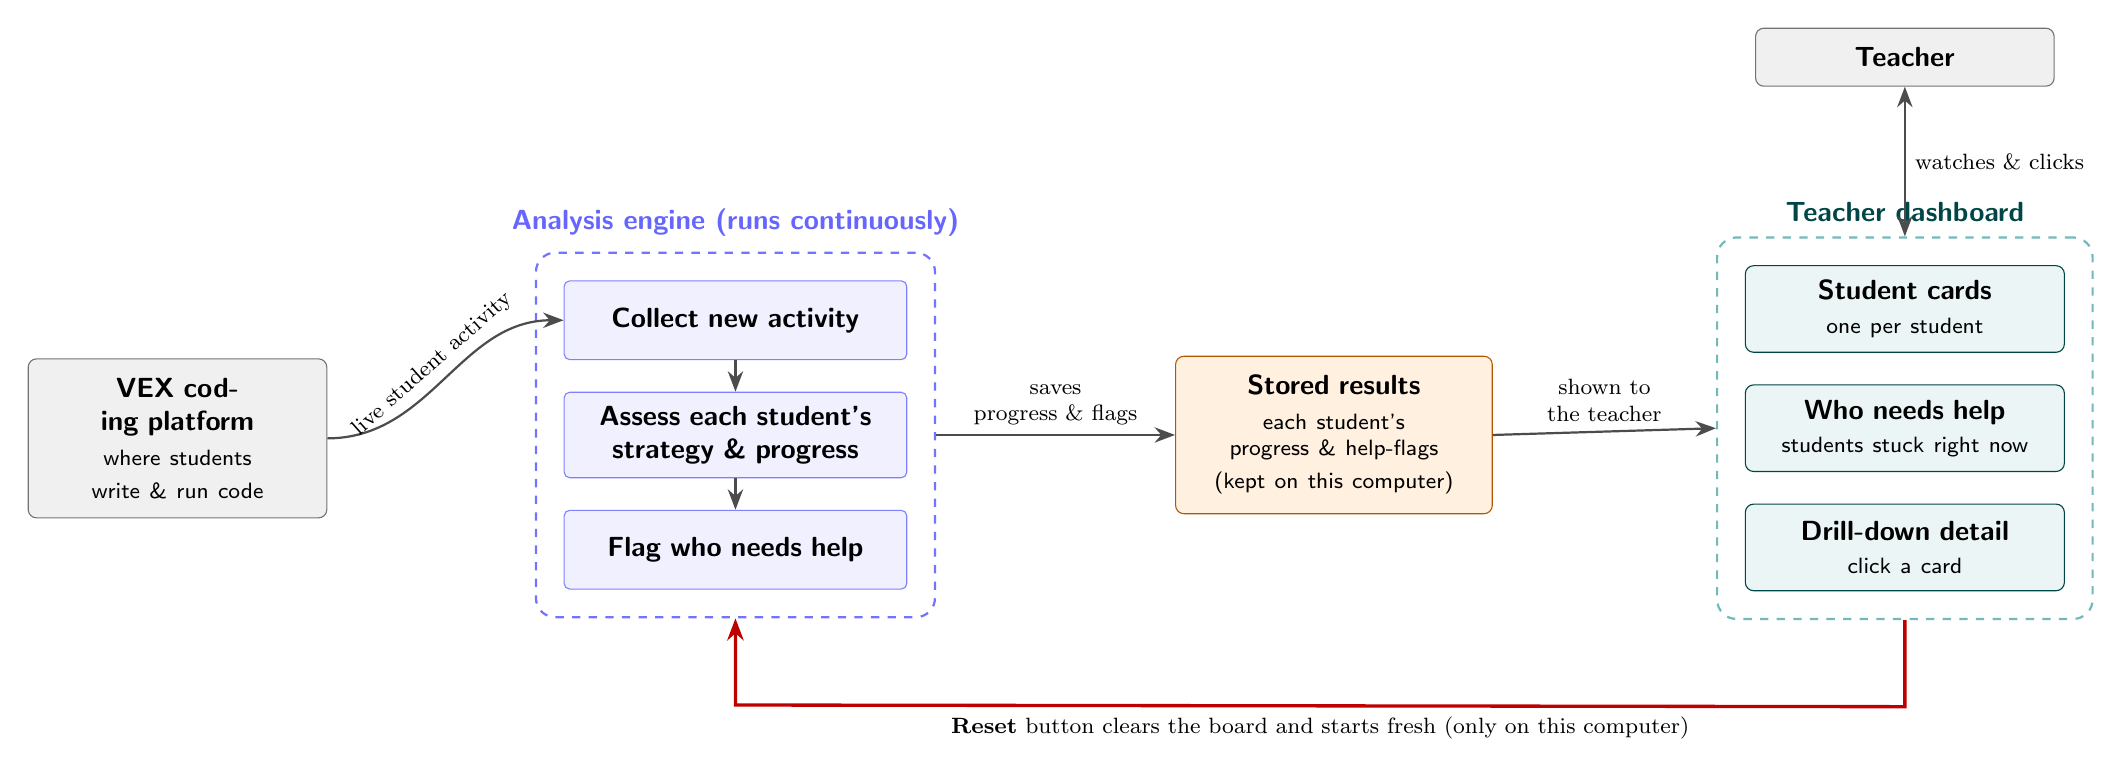
\begin{tikzpicture}[
  font=\sffamily, >=Stealth,
  ext/.style  ={rounded corners=3pt, draw=black!55, fill=black!6,  align=center, inner sep=7pt, text width=33mm},
  ebox/.style ={rounded corners=2pt, draw=blue!50,  fill=blue!6,   align=center, inner sep=5pt, text width=40mm, minimum height=10mm},
  store/.style={rounded corners=3pt, draw=orange!70!black, fill=orange!12, align=center, inner sep=6pt, text width=36mm, minimum height=20mm},
  pane/.style ={rounded corners=3pt, draw=teal!55!black, fill=teal!8, align=center, inner sep=5pt, text width=37mm, minimum height=11mm},
  grp/.style  ={rounded corners=7pt, draw=#1, thick, dashed, inner sep=10pt},
  flow/.style ={-{Stealth[length=2.6mm]}, thick, draw=black!70},
  bi/.style   ={{Stealth[length=2.6mm]}-{Stealth[length=2.6mm]}, thick, draw=black!70},
  reset/.style={-{Stealth[length=2.8mm]}, very thick, draw=red!75!black},
]

% ---------- VEX platform ----------
\node[ext] (vex) {\textbf{VEX coding platform}\\[3pt]\footnotesize where students\\ write \& run code};

% ---------- Analysis engine ----------
\node[ebox, right=30mm of vex, yshift=15mm] (collect) {\textbf{Collect new activity}};
\node[ebox, below=4mm of collect]           (assess)  {\textbf{Assess each student's}\\\textbf{strategy \& progress}};
\node[ebox, below=4mm of assess]            (flag)    {\textbf{Flag who needs help}};
\draw[flow] (collect)--(assess); \draw[flow] (assess)--(flag);
\begin{scope}[on background layer]
  \node[grp=blue!55, fit=(collect)(assess)(flag)] (engine) {};
\end{scope}
\node[blue!60, font=\sffamily\bfseries, above=2pt of engine] {Analysis engine (runs continuously)};

% ---------- Stored results ----------
\node[store, right=34mm of assess] (store) {\textbf{Stored results}\\[3pt]\footnotesize each student's\\ progress \& help-flags\\ (kept on this computer)};

% ---------- Teacher dashboard ----------
\node[pane, right=32mm of store, yshift=16mm] (cards) {\textbf{Student cards}\\\footnotesize one per student};
\node[pane, below=4mm of cards]               (need)  {\textbf{Who needs help}\\\footnotesize students stuck right now};
\node[pane, below=4mm of need]                (detail){\textbf{Drill-down detail}\\\footnotesize click a card};
\begin{scope}[on background layer]
  \node[grp=teal!55, fit=(cards)(need)(detail)] (dash) {};
\end{scope}
\node[teal!55!black, font=\sffamily\bfseries, above=2pt of dash] {Teacher dashboard};

% ---------- Teacher ----------
\node[ext, above=19mm of dash] (teacher) {\textbf{Teacher}};

% ---------- flows ----------
\draw[flow] (vex.east) to[out=0,in=180] node[above, font=\footnotesize, sloped]{live student activity} (collect.west);
\draw[flow] (engine.east) -- node[above, font=\footnotesize, align=center]{saves\\ progress \& flags} (store.west);
\draw[flow] (store.east) -- node[above, font=\footnotesize, align=center]{shown to\\ the teacher} (dash.west);
\draw[bi]   (teacher.south) -- node[right, font=\footnotesize]{watches \& clicks} (dash.north);

% ---------- reset (plain) ----------
\draw[reset] (dash.south) -- ($(dash.south)+(0,-11mm)$)
  -- node[below, font=\footnotesize, align=center]
       {\textbf{Reset} button clears the board and starts fresh (only on this computer)}
     ($(engine.south)+(0,-11mm)$)
  -- (engine.south);

\end{tikzpicture}
\end{document}
